\documentclass[11pt,oneside]{book}

\usepackage{xcolor}                    % For creating coloured text and background

\usepackage{xcolor}
\usepackage{titlesec}
\usepackage{mdframed}
\usepackage{wrapfig}

\colorlet{rulercolor}{gray!50}

\titleformat{\chapter}
  {\normalfont\sffamily\Large\fontfamily{phv}\selectfont}
  {\thechapter.}{.5em}{}
  [\vspace{.2ex}\color{rulercolor}\titlerule]
  
\newmdenv[leftmargin=20pt, rightmargin=20pt, 
skipabove=\topsep,skipbelow=\topsep,
backgroundcolor=gray!30,shadow=true,shadowsize=4,
roundcorner=10pt]{shadebox}

\newmdenv[leftmargin=30pt, rightmargin=30pt, 
skipabove=0pt,skipbelow=0pt,
backgroundcolor=gray!20]{mybox}

\usepackage{graphicx}
%%	using final option to force graphics to be included even in draft mode
%\usepackage[final]{graphicx}
\usepackage{paralist} % compact lists

%% Support sub-figures.
\usepackage{subfigure}

%% Make subsections numbered and included in ToC
\setcounter{secnumdepth}{3}
\setcounter{tocdepth}{2}

%% Make margins less ridiculous
\usepackage[margin=1.2in]{geometry}

%% Package to linebreak URLs in a sane manner.
\usepackage{url}

%% Define a new 'smallurl' style for the package that will use a smaller font.
\makeatletter
\def\url@smallurlstyle{%
  \@ifundefined{selectfont}{\def\UrlFont{\sf}}{\def\UrlFont{\small\ttfamily}}}
\makeatother
%% Now actually use the newly defined style.
\urlstyle{smallurl}
%% Make URLs clickable
\usepackage[colorlinks, bookmarks=true]{hyperref}
\usepackage[all]{hypcap}


%% Since I'm using the LaTeX Makefile that uses dvips, I need this
%% package to make URLs break nicely
\usepackage{breakurl}

\usepackage{array}

%% Make table cross pages.
\usepackage{longtable}

%% Make links to captions point to the figure, not just the caption at bottom
\usepackage[all]{hypcap}

% create a shortcut to typeset table headings
\newcommand\tabhead[1]{\small\textbf{#1}}

\graphicspath{{figures/}} 
\DeclareGraphicsExtensions{.eps}

\setlength{\headheight}{15.2pt}

\usepackage{fancyhdr}
\pagestyle{fancy}
  \renewcommand{\chaptermark}[1]{\markboth{\MakeUppercase{\chaptername \ \thechapter \ \ #1}}{}}
  \fancyhf{}%clear all header and footer fields
    \fancyhead[LO]{\nouppercase{\rightmark}}
    \fancyhead[RE]{\nouppercase{\leftmark}}
       \fancyhead[RO,LE]{\thepage}
\def\chem#1#2{{{\scriptscriptstyle#1\atop\longrightarrow}\atop{\longleftarrow\atop\scriptscriptstyle#2}}}

\title{\textbf{Serious Game Stakeholder Experience Assessment Method (SGSEAM) \\
User Guide}}

\author{Yongwen Xu, Philip M. Johnson, Carleton A. Moore, Robert S. Brewer\\
\\
\em  Collaborative Software Development Laboratory \\
\em  Department of Information and Computer Sciences \\
\em  University of Hawai'i at Manoa\\
     \{yxu, johnson, cmoore, rbrewer\}@hawaii.edu}

\date{\today}

\begin{document}
  \maketitle
  \thispagestyle{empty}
  \tableofcontents
  \newpage
  
\chapter{SGSEAM Overview}
One of the benefits of using a serious game framework is that, if correctly designed, it will 
provide useful and reusable ``building blocks'' with which to develop a variety of serious 
games. Yet how are we to know if a serious game framework has been ``correctly designed''?

Serious Game Stakeholder Experience Assessment Method (SGSEAM) describes a method for 
assessing serious game frameworks from the stakeholder 
experience perspectives.  The goal of SGSEAM is to identify (a) major strengths of a serious game
framework, which aids the community by indicating features of the framework to emulate, and
(b) major shortcomings of the framework, which aids the community by indicating features to avoid.
The benefits of SGSEAM assessment are for the developers of serious game frameworks 
to learn and improve from the findings of the assessment.

SGSEAM is an assessment method instead of an evaluation method. The main purpose 
of an evaluation is to determine the quality of a program by formulating a judgment. An assessment, on 
the other hand, is nonjudgmental. SGSEAM does not try to judge a framework according to a 
standard, or to compare one framework against another. Instead, it is used to identify the major 
strengths and shortcomings of a framework to benefit  the developers of the framework.

\autoref{fig:overview} outlines the steps of the process of applying SGSEAM to a framework.

\begin{figure}[ht!]
  \center
  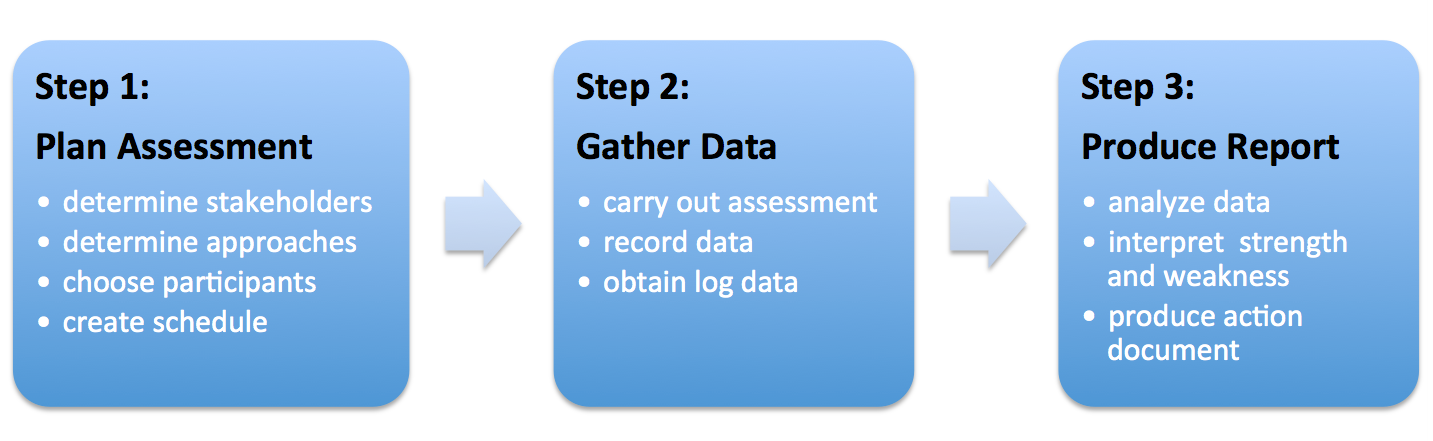
\includegraphics[width=0.8\columnwidth]{sgseam-steps}
  \caption{Applying SGSEAM to a framework}
  \label{fig:overview}
\end{figure}

There are three steps in the process of applying SGSEAM. Step one is to plan the assessment, including identifying the stakeholder and participants and creating the assessment plan. The deliverable for this step is the assessment plan document. Step two is to gather data. The deliverable for this step is the assessment data repository. Step three is to produce the strength and weakness report. The deliverable for this step is the action document for framework improvement. The following chapters describe the steps in details.

\chapter{Plan Assessment}

\section{Identify stakeholders}

\begin{shadebox}
\begin{wrapfigure}{l}{0.04\textwidth}
\vspace{-15pt}\hspace{-10pt}
    
\includegraphics[width=0.04\textwidth]{note-icon}
\end{wrapfigure}

Identify the stakeholders in each SGSEAM stakeholder class, write down their names and roles.

\end{shadebox}

SGSEAM assesses the experiences for the stakeholders listed in \autoref{table:stakeholders}. For each stakeholder, identify the population, the name and contact if possible. It is important to be able to contact the stakeholders in some way, either via email or phone, to get the feedback from their experiences with the framework.

\begin{table}[ht!]
  \centering
  \begin{tabular}{|c|c|c|}
    \hline
    \multicolumn{1}{|p{0.22\columnwidth}|}{\centering\tabhead{Stakeholder class}} &
    \multicolumn{1}{|p{0.4\columnwidth}|}{\centering\tabhead{Definition}} &
    \multicolumn{1}{|p{0.28\columnwidth}|}{\centering\tabhead{Examples}} \\
    \hline
    \multicolumn{1}{|p{0.22\columnwidth}|}{Players} &
    \multicolumn{1}{|p{0.4\columnwidth}|}{participate in the game produced by the framework.} &
    \multicolumn{1}{|p{0.28\columnwidth}|}{students, residents} \\
    \hline
    \multicolumn{1}{|p{0.22\columnwidth}|}{System admins} &
    \multicolumn{1}{|p{0.4\columnwidth}|}{install and maintain the technological game infrastructure.} &
    \multicolumn{1}{|p{0.28\columnwidth}|}{system admin, IT staffs} \\
    \hline
    \multicolumn{1}{|p{0.22\columnwidth}|}{Game designer} &
    \multicolumn{1}{|p{0.4\columnwidth}|}{design the content and game mechanics.} &
    \multicolumn{1}{|p{0.28\columnwidth}|}{instructional designers, content experts} \\
    \hline
    \multicolumn{1}{|p{0.22\columnwidth}|}{Game managers} &
    \multicolumn{1}{|p{0.4\columnwidth}|}{manage the game during the period of game play.} &
    \multicolumn{1}{|p{0.28\columnwidth}|}{sustainability coordinators, residential staffs} \\
    \hline
    \multicolumn{1}{|p{0.22\columnwidth}|}{Game developers} &
    \multicolumn{1}{|p{0.4\columnwidth}|}{develop customization, extend and enhance the game.} &
    \multicolumn{1}{|p{0.28\columnwidth}|}{programmers, internal developers} \\
    \hline
  \end{tabular}
  \caption{SGSEAM Stakeholders}
  \label{table:stakeholders}
\end{table}

\section{Determine assessment approach}

\begin{shadebox}
\begin{wrapfigure}{l}{0.04\textwidth}
\vspace{-15pt}\hspace{-10pt}
    
\includegraphics[width=0.04\textwidth]{note-icon}
\end{wrapfigure}
Determine the appropriate assessment approaches for each stakeholder.
\end{shadebox}

There are usually multiple assessment approaches for each stakeholder.  \autoref{table:approaches} provides an overview of the assessment method and the approaches. The appropriate assessment approaches should be determined according to the resource available. The approaches for a stakeholder is additive.The more approaches applied, the higher confidence of the assessment can be achieved. 

\begin{table}[ht!]
  \centering
  \begin{tabular}{|c|c|c|}
    \hline
    \multicolumn{1}{|p{0.18\columnwidth}|}{\centering\tabhead{Stakeholder}} &
    \multicolumn{1}{|p{0.28\columnwidth}|}{\centering\tabhead{Assessment Goal}} &
    \multicolumn{1}{|p{0.45\columnwidth}|}{\centering\tabhead{Assessment approaches}} \\
    \hline
    \multicolumn{1}{|p{0.18\columnwidth}|}{Player} &
    \multicolumn{1}{|p{0.28\columnwidth}|}{How does the framework affect and engage players?} &
    \multicolumn{1}{|p{0.45\columnwidth}|}{
    	Pre-post effectiveness study(\ref{Pre-Post effectiveness study});\newline
	Self-reported usability metrics(\ref{Self-reported usability metrics});\newline
	Engagement metrics(\ref{Engagement metrics})} \\
    \hline
    \multicolumn{1}{|p{0.18\columnwidth}|}{System admin} &
    \multicolumn{1}{|p{0.28\columnwidth}|}{How easy is it to install and maintain the system?} &
    \multicolumn{1}{|p{0.45\columnwidth}|}{
    	Post-hoc system admin interview(\ref{Post-hoc system admin interview});\newline
	In-lab installation study(\ref{In-lab installation study})} \\
    \hline
    \multicolumn{1}{|p{0.18\columnwidth}|}{Game designer} &
    \multicolumn{1}{|p{0.28\columnwidth}|}{How easy is it to design a game?} &
    \multicolumn{1}{|p{0.45\columnwidth}|}{
    	Post-hoc designer interview(\ref{Post-hoc game designer interview});\newline
	In-lab game design study(\ref{In-lab game design study})}\\
    \hline
    \multicolumn{1}{|p{0.18\columnwidth}|}{Game manager} &
    \multicolumn{1}{|p{0.28\columnwidth}|}{How easy is it to manage a game?} &
    \multicolumn{1}{|p{0.45\columnwidth}|}{
    	Post-hoc manager interview(\ref{Post-hoc game manager interview});\newline
	In-lab game management study(\ref{In-lab game management study})}\\
    \hline
    \multicolumn{1}{|p{0.18\columnwidth}|}{Game developer} &
    \multicolumn{1}{|p{0.28\columnwidth}|}{How easy is it to enhance the system?} &
    \multicolumn{1}{|p{0.45\columnwidth}|}{
    	Post-hoc developer interview(\ref{Post-hoc game developer interview});\newline
	In-lab game development study(\ref{In-lab game development study})} \\
    \hline
  \end{tabular}
  \caption{SGSEAM approaches}
  \label{table:approaches}
\end{table}

The assessment approaches is categorized into in-vivo and in-vitro assessments. The in-vivo approaches, such as pre-post test, in-game surveys and post-hoc interviews, assess the real world instance of the game. The in-vitro approaches use in-lab experiments in a simulated environment. Different assessment
approaches will have different levels of rigor or validity. For example, the in-lab experiments (in-vitro) can enlist several subjects to perform the same pre-defined tasks and collect comparable data in a more controlled setting, while in-game surveys or interviews in the in-vivo approach typically collect data from different settings but the data reflect the real world interaction between the stakeholders and the framework.

The following sections describe in detailed the different approaches for each stakeholder.  Each assessment approach describes the goal of the assessment, what data to collect, how to collect the data and how to analyze the data to obtain insights about the strengths and weaknesses of the framework from each stakeholder's perspective.

\subsection{Player assessment}

The goal of player assessment is to determine the effectiveness of the game
framework from player's perspective. It is essential that a game produced by a serious game
framework could achieve its intended "serious" purpose. The intended purposes of serious games are
always subject specific. For example, the desired effect of a serious game for
energy education and conservation is to increases players' energy literacy and
reduces their energy consumption during (and, hopefully, after) the game. A serious game for
language learning would have a very different desired effect.

\subsubsection{Player assessment approach: Pre-Post effectiveness study}
\label{Pre-Post effectiveness study}

This approach requires users of SGSEAM to first determine a set of domain-specific questions to assess the 
desired effects of their serious game. For example, a set of questionnaires on sustainability literacy, such as knowledge of power and energy, is used to assess the effectiveness of a serious game for sustainability education.

Once the domain-specific questionnaires are determined and designed, present this questionnaires as a survey to a random selection of the players before the game starts. After the game ends, present the same survey to the
same players again. Compare the two set of survey response data to study if the game has an impact on the players regarding to the survey subjects. The extent of the changes reflected in the survey result indicates the degree of effectiveness of the serious game for this subject.

Serious games often engage players with resources of various types (energy, water, waste, etc.). Collect these measurements before, during, and after the game in order to acquire evidence regarding the potential impact upon player use of these resources.

\subsubsection{Player assessment approach: Self-reported usability metrics}
\label{Self-reported usability metrics}

This approach interviews players about their self-reported experiences with the game. The interview could be administrated via a face-to-face conversation or through 
online survey. We found that the online survey is more cost effective than face-to-face conversation. 
In additions, the online survey could be implemented as an activity inside the game. For example, the Makahiki serious game framework implements a survey activity which incentivizes players to complete the survey by rewarding game points for the activity.

Use the usability questionnaires in \autoref{fig:usability-metrics} to interview players:\\

\begin{figure}[ht!]
\begin{mybox}
\begin{compactenum}
\item What did you like most about the game?
\item What did you found confusing?
\item What issues did you have while using the game?
\item What was the thing you liked the least about the game?
\item What can we do to improve the game?
\item It was easy to find what I was looking for on the website.  \\
	Strongly disagree  -  Disagree  -  Neutral  -  Agree  -  Strongly agree
\item The website was responsive. \\
	Strongly disagree  -  Disagree  -  Neutral  -  Agree  -  Strongly agree
\item The website provided adequate help in teaching me how to play. \\
	Strongly disagree  -  Disagree  -  Neutral  -  Agree  -  Strongly agree
\item I understood how to play. \\
	Strongly disagree  -  Disagree  -  Neutral  -  Agree  -  Strongly agree
\item this is something my friends should participate in. \\
	Strongly disagree  -  Disagree  -  Neutral  -  Agree  -  Strongly agree
\end{compactenum}
\end{mybox}
\caption{Player self-reported usability metrics questionnaires}
\label{fig:usability-metrics}  
\end{figure}


\subsubsection{Player assessment approach: Engagement metrics}
\label{Engagement metrics}

Player engagement is an important measure for understanding the effectiveness of a serious game.
Engagement metrics assess the extent of participation by players and the impact of the game. 

Calculate as many as possible the player engagement metrics described in \autoref{table:engagement-metrics} by analyzing the data from system log or other channels provided by the framework. The more metrics obtained, the better understanding of the extent of player engagement.

\begin{table}[ht!]
  \centering
  \begin{tabular}{|c|c|c|}
    \hline
    \multicolumn{1}{|p{0.2\columnwidth}|}{\centering\tabhead{Metric}} &
    \multicolumn{1}{|p{0.3\columnwidth}|}{\centering\tabhead{Definition}} &
    \multicolumn{1}{|p{0.35\columnwidth}|}{\centering\tabhead{Mesure}} \\
    \hline
    \multicolumn{1}{|p{0.2\columnwidth}|}{participation} &
    \multicolumn{1}{|p{0.3\columnwidth}|}{percentage of players who play the game} &
    \multicolumn{1}{|p{0.35\columnwidth}|}{the level of involvement from players} \\
    \hline
    \multicolumn{1}{|p{0.2\columnwidth}|}{player} &
    \multicolumn{1}{|p{0.3\columnwidth}|}{number of players per day} &
    \multicolumn{1}{|p{0.35\columnwidth}|}{the frequency of players interact with the game} \\
    \hline
    \multicolumn{1}{|p{0.2\columnwidth}|}{play time} &
    \multicolumn{1}{|p{0.3\columnwidth}|}{play time of a player per day} &
    \multicolumn{1}{|p{0.35\columnwidth}|}{the frequency of players interact with the game} \\
    \hline
    \multicolumn{1}{|p{0.2\columnwidth}|}{submission} &
    \multicolumn{1}{|p{0.3\columnwidth}|}{submissions of all player per day} &
    \multicolumn{1}{|p{0.35\columnwidth}|}{the rate of players' completion of game activities} \\
    \hline
    \multicolumn{1}{|p{0.2\columnwidth}|}{social interaction} &
    \multicolumn{1}{|p{0.3\columnwidth}|}{social interaction of all player per day} &
    \multicolumn{1}{|p{0.35\columnwidth}|}{the rate of in-game social interactions between players} \\
    \hline
    \multicolumn{1}{|p{0.2\columnwidth}|}{game error} &
    \multicolumn{1}{|p{0.3\columnwidth}|}{game errors per day} &
    \multicolumn{1}{|p{0.35\columnwidth}|}{the rate of errors encountered by players during the game} \\
    \hline
  \end{tabular}
  \caption{Player engagement metrics}
  \label{table:engagement-metrics}
\end{table}

With the exception of the game error metric, the higher value these metrics are, the higher engagement level the game has.

\subsection{System admin assessment}

System administrators are responsible for installing and maintaining the software infrastructure
for the game. Their tasks include the framework and dependency installation, maintain the database, backups, and so forth.

\subsubsection{System admin assessment approach: Post-hoc admin interview}
\label{Post-hoc system admin interview}

One approach to assess the question of how easy it is to install and maintain the system is a post-hoc interview. The actual system admin(s) are asked about their experience after their installation in the production system. The interview includes the following questions:\\

\begin{figure}[ht!]
\begin{mybox}
\begin{compactenum}
\item How much time did you require to install the system and the dependencies?
\item How much time did you require to maintain the system?
\item What problems did you encounter?
\item Did you find it difficult to admin the system? What was difficult?
\end{compactenum}
\end{mybox}
\caption{System admin interview questionnaires}
\label{fig:system-admin-interview}  
\end{figure}

After the interview data is acquired, the assessor will perform qualitative data
analysis, which involves transcribing (if the interview data is in audio format),
categorizing and coding the description of reported problems or difficulties.

\subsubsection{System admin assessment approach: In-lab installation study}
\label{In-lab installation study}

Another approach to assess the question is to use an in-lab experimental study. A group of system admins will 
be asked to install the system, record the time
spent and problem encountered as they complete each step. The qualitative data (i.e., the
descriptive problems reported by the participants of the study) will need to be categorized and
coded. The assessor will triangulate the reported time data and the problem categories to identify
the area of strength (less time spent) and weakness (problems and difficulties).

The level of confidence of the above two assessment approaches varies. The experimental study
approach is more rigor because of the generality achieved from the larger population of
participants under study. The data collected during the step by step experimental study is more
accurate than the one collected in the post-hoc interview.

\subsection{Game designer assessment}

A game designer uses the serious game framework to design and create a serious game.
A serious game framework always provides certain tools or interfaces to game designers
with the hope that these will simplify the design of a game. Such tools might involve
configuring global settings for the game, such as how long will the game run, who are the
players, and how to design individual game elements.

SGSEAM assesses the game designer stakeholder by addressing the following two questions: (a) How
much time is required to design an instance of a serious game using the framework? and (b) How
many, and how problematic are the errors that designers encounter during the design process?

There are three approaches for game designer assessment:

\subsubsection{Game designer assessment approach: Post-hoc designer interview}
\label{Post-hoc game designer interview}

One approach is to interview the actual game designer(s) after they had completed the design in a production system. The following questions will be asked:\\
 
\begin{figure}[ht!]
\begin{mybox}
\begin{compactenum}
\item How much time did you spend to complete each design task?
\item What problems did you encounter?
\item Did you find it difficult to configure? What was difficult?
\item Did you find it difficult to design a specific game? Which one, and what was difficult?\\
\end{compactenum}
\end{mybox}
\caption{Game designer interview questionnaires}
\label{fig:game-designer-interview}  
\end{figure}

The interview data will be transcribed (if audio recording), categorized and coded to identify the
strengths and weaknesses.

Collect the system log data related to the game designing tasks. When
available, the time spent and error encountered can be queried from the system logs. Although these
system generated data might be easier to gather in some systems, it might not provide the same
depths or insights than the other two approaches where the experiences are provided by the
participants directly. On the other hand, these system data can be supplemental to the other
approaches. They could be correlated with the data gathered from the other assessment approaches
 to increase the confident of the assessment.

\subsubsection{Game designer assessment approach: In-lab game design study}
\label{In-lab game design study}

Another approach is an in-lab experimental study, where a
goup of participants is asked to use the system to perform a same set of design tasks. The time
spent and problems encountered are recorded for each tasks. The assessor will triangulate the
reported time data and the problem categories to identify the strengths and weaknesses.

\subsection{Game manager assessment}

A game manager uses the serious game framework to manage the serious game that the game
designers created. It is possible that a game manager is also the game designer.
Serious game frameworks normally provide certain interfaces for the managers to manage the
game. This may involve managing player submissions, monitoring the game state, entering
manual resource data, notifying winners of the game, etc.

SGSEAM assesses the game manager stakeholder with the following questions: (a) How much time is
required to manage an instance of a serious game using the framework? and (b) How many,
and how problematic are the errors that managers encounter during the design process?

Similar to the assessment of game designer experience, SGSEAM proposes three approaches. 

\subsubsection{Game manager assessment approach: Post-hoc manager interview}
\label{Post-hoc game manager interview}

The post-hoc interview approach gather data from the game manger(s) by asking the following questions:\\
 
\begin{figure}[ht!]
\begin{mybox}
\begin{compactenum}
\item How much time did you spend to complete each managing task?
\item What problems did you encounter?
\item Did you find it difficult to manage? What was difficult?\\
\end{compactenum}
\end{mybox}
\caption{Game manager interview questionnaires}
\label{fig:game-manager-interview}  
\end{figure}

The log data analysis collects system log data related to the game managing tasks. The time spent and error encountered can be deducted from the system log and reveals strengths and weaknesses of the game managing interface.

\subsubsection{Game manager assessment approach: In-lab game management study}
\label{In-lab game management study}

The experimental study approach gather data from a group of participants about the time spent and
problems encountered for each task of managing the serious game. 

\subsection{Game developer assessment}

The game developer stakeholder is different from the game designer stakeholder, in that the
game designer stakeholder tailors the framework without requiring any software
development, while the game developer stakeholder enhances, corrects, and extends the system by
manipulating code. 

To investigate how easy it is to understand, extend, and debug a serious game
framework from a developer's perspective, SGSEAM assesses how much time it takes to develop an
enhancement to the game framework, and how many errors are encountered
during the process.

\subsubsection{Game developer assessment approach: Post-hoc developer interview}
\label{Post-hoc game developer interview}

This assessment approach is accomplished by interviewing the actual developer(s) to
answer the following questions:\\
 
\begin{figure}[ht!]
\begin{mybox}
\begin{compactenum}
\item How much time did you spend developing a customization using the game framework?
\item What problem(s) did you encounter?
\item Did you find it difficult to understand, extend and debug the system? What was difficult?\\
\end{compactenum}
\end{mybox}
\caption{Game developer interview questionnaires}
\label{fig:game-developer-interview}  
\end{figure}

\subsubsection{Game developer assessment approach: In-lab game development study}
\label{In-lab game development study}

The experimental study assessment approach asks a group of developers to develop a same set of
enhancements to the system, and ask them to record the time spent to develop and problems
encountered during the development.

Similarly, the descriptive data will be categorized and coded. The time data will be correlated to the problem data to identify the areas of strength and weakness.

\section {Choose participants}
\begin{shadebox}
\begin{wrapfigure}{l}{0.04\textwidth}
\vspace{-15pt}\hspace{-10pt}
    
\includegraphics[width=0.04\textwidth]{note-icon}
\end{wrapfigure}
Choose participants from each stakeholder class.
\end{shadebox}

\section{Create assessment schedule}
\begin{shadebox}
\begin{wrapfigure}{l}{0.04\textwidth}
\vspace{-15pt}\hspace{-10pt}
    
\includegraphics[width=0.04\textwidth]{note-icon}
\end{wrapfigure}
Create a schedule for each assessment, produce the assessment planning document.
\end{shadebox}

\chapter{Gather Data}
This step carries out the assessment, record the data, obtain log data, and refine the assessment plan if necessary. The output of this step is a data repository contains all the assessment data that can be analyzed in the next step.

\section{Carry out the assessment}
\begin{shadebox}
\begin{wrapfigure}{l}{0.04\textwidth}
\vspace{-15pt}\hspace{-10pt}
    
\includegraphics[width=0.04\textwidth]{note-icon}
\end{wrapfigure}
Carry out the assessment.
\end{shadebox}

\section{Record data}
\begin{shadebox}
\begin{wrapfigure}{l}{0.04\textwidth}
\vspace{-15pt}\hspace{-10pt}
    
\includegraphics[width=0.04\textwidth]{note-icon}
\end{wrapfigure}
Record the data from the assessment.
\end{shadebox}

\section{Obtain log data}
\begin{shadebox}
\begin{wrapfigure}{l}{0.04\textwidth}
\vspace{-15pt}\hspace{-10pt}
    
\includegraphics[width=0.04\textwidth]{note-icon}
\end{wrapfigure}
Obtain the log data from the framework, including all the interaction log from the each stakeholder.
\end{shadebox}

\chapter{Produce Strength and Weakness report}

Analyze the data and produce the action report.

\section{Analyze data}
\begin{shadebox}
\begin{wrapfigure}{l}{0.04\textwidth}
\vspace{-15pt}\hspace{-10pt}
    
\includegraphics[width=0.04\textwidth]{note-icon}
\end{wrapfigure}
Analyze the data from the data repository.
\end{shadebox}

\section{Interpret strength and weakness of framework}
\begin{shadebox}
\begin{wrapfigure}{l}{0.04\textwidth}
\vspace{-15pt}\hspace{-10pt}
    
\includegraphics[width=0.04\textwidth]{note-icon}
\end{wrapfigure}
Interpret strength and weakness of framework.
\end{shadebox}

\section{Produce artifact action document}
\begin{shadebox}
\begin{wrapfigure}{l}{0.04\textwidth}
\vspace{-15pt}\hspace{-10pt}
    
\includegraphics[width=0.04\textwidth]{note-icon}
\end{wrapfigure}
Produce artifact action document.
\end{shadebox}

%% Use this for an alphabetically organized bibliography
%%\bibliography{sustainability,csdl-trs,gamification,yxu}
%%\bibliographystyle{plain}

\end{document}